\subsubsection{Метод Аббе}
Работаем все с теми же понятиями. 
Сначала за объект возьмём дифракционную решетку. 
Так же при падении параллельных лучей монохроматического света у нас до какого-то порядка максимума будут однородные волны, а дальше неоднородными, которые затухая, на расстояниях порядка $\lambda$ в наш объектив не попадут.

Поставим перед объективом диафрагму, пропускающую определенные порядки спектров. Например, если пропускается лишь нулевой, то о решетке(объекте) мы никакой информации не получим, а в плоскости изображения получим равномерно освещенное поле.

Поэтому возьмём диафрагму, пропускающую $m$ и $m+1$ порядки. Которые оставят только плоские волны, которые будут интерферировать между собой:
\begin{equation*}
	E_m = a_m \cos (\omega t - \vc{k}_m \vc{r}),
	\hspace{1 cm}
	E_{m+1} = a_{m+1} \cos (\omega t - \vc{k}_{m+1} \vc{r}).
\end{equation*}
Примем за плоскость решетки $XY$, волна распространяется в сторону $Z$. Посмотрим на какую-нибудь плоскость $z = \const$ и найдём расстояние между интерференционными полосами в ними:
\begin{equation*}
	\Delta \varphi = (k_{m+1, x} - k_{m, x}) \Delta x.
\end{equation*}
Видим, что интенсивность света будет периодически повторяться $\Delta \varphi = 2 \pi, 4 \pi, \ldots$ (типа саморепродукция). И шириной интерференционной полосы возьмём $\Delta x$ при $\Delta \varphi = 2 \pi$.

Направления на взятые максимумы:
\begin{equation*}
	d \cdot (\sin \vartheta_m -  \sin \theta) = m \lambda,
	\hspace{0.7 cm}
	d \cdot (\sin \vartheta_{m+1} -  \sin \theta) = (m+1) \lambda.
\end{equation*}
Так же знаем:
\begin{equation*}
	k_{m, x} = \left(\frac{2 \pi}{\lambda}\right) \sin \vartheta_m
	\hspace{0.7 cm}
	k_{m+1, x} = \left(\frac{2 \pi}{\lambda}\right) \sin \vartheta_{M+1}
\end{equation*}
Тогда получаем:
\begin{equation*}
	k_{m+1, x} - k_{m, x} = \left(\frac{2 \pi}{\lambda}\right)(\sin \vartheta_{m+1} - \sin \vartheta_m) = \frac{2 \pi}{d}.
\end{equation*}
Таким ширина полосы: $\Delta x = \frac{2 \pi}{2\pi d} = d$.
И экстраполируя не на ближайшие максимумы аналогично получаем
\begin{equation*}
	\Delta x = \frac{d}{\Delta m}.
\end{equation*}
Стоит обобщить, сказав, что чем больше дифрагированных волн различных порядков проходит через диафрагму, тем совершеннее получается изображение.

Решетка бралась как простейший объект, для которого хватает оставить наименее совершенное изображение, которое даст только понятие о её периодичности. Тогда оценим разрешающую способность объектива в который нормально попали 1ый и -1ый максимумы. Пусть у объектива ещё показатель преломления $n$. Минимальные период решетки, при котором:
\begin{equation*}
	 d \sin \alpha = \frac{\lambda}{n}
	 \hspace{1 cm}
	 \Rightarrow
	 \hspace{1 cm}
	 l_\text{мин} = \frac{\lambda}{n \sin \alpha}.
\end{equation*}
Нормальная такая оценка получилось, с точностью до домножения на константу порядка единицы.

Упрощение связанное с рассмотрением объекта-решетки не принципиально. За объектом произвольной формы возникнут самые разные дифрагировавшие пучки.
Угол дифракционной расходимости на первый минимум будет таким, что
\begin{equation*}
	n l \sin \vartheta \sim \lambda,
\end{equation*}
для $l$ -- линейного размера объекта.
Минимальные же размеры объекта для лучей падающих под углом $\alpha$ будет определятся условием $\vartheta \sim \alpha$, а именно опять
\begin{equation*}
	l_\text{min} \sim \frac{\lambda}{n \sin \alpha}.
\end{equation*}

О чем же думал Аббе? Что давайте смотреть на изображения, которые даёт нам линза в такой же манере (или любой другой оптический прибор).
\begin{figure}[ht]
    \centering
    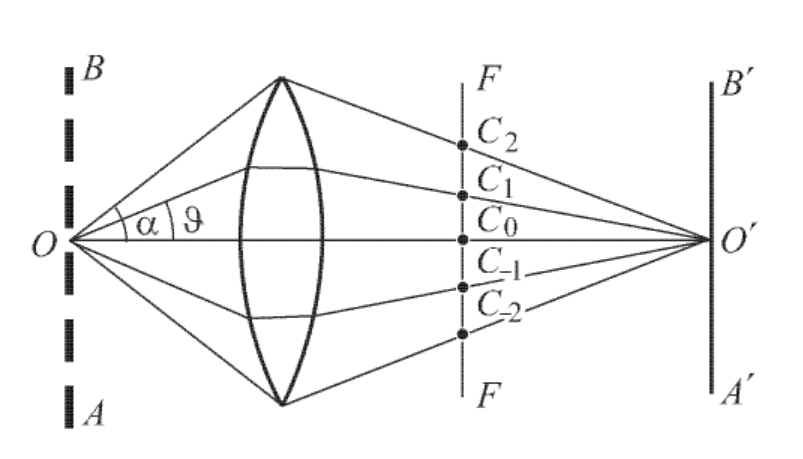
\includegraphics[width=0.45\textwidth]{figures/220.png}
    %\caption{}
    %\label{fig:}
\end{figure}
В фокусе мы получаем дифракционную картину из точек $C_k$, которую Аббе назвал первичным изображением объекта. Далее по Гюйгенсу-Френелю можно рассчитать световое поле далее за фокальной плоскостью, пусть они соберутся нашим объективом хоть где-то дальше, тогда получим \textit{вторичное изображение} или \textit{вторичную дифракцию}.
